% !TEX root = main.tex

\chapter{Theoretical framework}
Quantum computing is based on a general framework that does not depend on the physical platform. Here, important concepts such as qubit, and quantum operations are described from a theoretical point of view, before showing how we can realize them with trapped ions. The same goes with quantum networking, the concept and the realization can be treated separately and they will be described in this chapter. Furthermore, in this chapter we will take a look into Gaussian beams and their properties. Since that is the shape emitted by laser, it is important to understand their characteristic and how to manipulate them. Lastly, Acousto-optical interactions are introduced and studied to give an idea of how AODs work and how they can be used to steer a laser beam.
\section{Quantum logic with trapped ions}
\subsection{Quantum computer and quantum gates}
The concepts of quantum computing are borrowed and extended from classical computational theory. In the classical case, information is mostly represented in terms of binary digits, the so called bit, essentially mapping information to a base-2 number. Information processing is done with gates acting of those numbers. The idea of quantum computer is still to encode information in a binary form, but due to the nature of quantum mechanics, a quantum bit (in short qubit) gains new features that can be exploited to perform different kind of operations.\\
A qubit is formally a normalized wave function that can be written as superposition of two orthogonal states indicated usually with $\ket{0}$ and $\ket{1}$:
\begin{equation}
\label{qubit}
\ket{\psi} = \alpha \ket{0} + \beta\ket{1},
\end{equation}
where $\alpha,\beta$ are probability amplitudes, two complex numbers that satisfy the relationship $|\alpha|^2+|\beta|^2 = 1$.
At first glance, the advantage of qubits seems obvious, while one classical bit can store only one bit of information, a qubit can be in any linear combination, i.e. $\alpha$ and $\beta$ can be chosen freely and any information can be represented. Although, the reality is different, due to rules of quantum mechanics, $\alpha$ and $\beta$ cannot be directly accessed, which means that we can get only a limited amount of information out of a qubit. The outcome of measuring a qubit will give the value 0 with a probability of $|\alpha|^2$ and 1 with a probability of $|\beta^2|$.\\
Qubits also have a geometrical representation that can be useful, equation \eqref{qubit} depends on 4 real numbers, however since $\psi$ is normalized, we can rewrite the expression as
\begin{equation}
\ket{\psi} = e^{i\gamma}\left(\cos\frac{\theta}{2}\ket{0} + e^{i\varphi}\sin\frac{\theta}{2}\ket{1}\right).
\end{equation}
the global phase factor $e^{i\gamma}$ can be left out, as it does not influence the measurement outcome. This leaves us with only two real number: $\theta$ and $\varphi$. A qubit is therefore representable with only these two numbers that we can chose to represent geometrically with normalized spherical coordinates. The so called Bloch sphere is depicted in figure \ref{blochsphere}, every point on its surface represents a different state of the qubit. Here qubit manipulation can be visualized as trajectories on the surface. The drawback of this representation is that it is limited to only one qubit, so it loses usefulness when dealing with multiple qubits.
\begin{figure}[H]
\centering
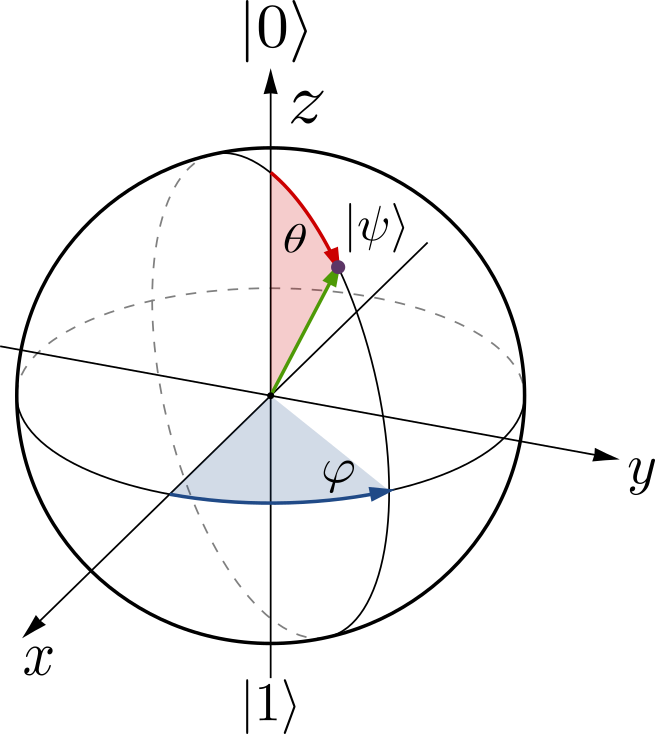
\includegraphics[width = .4\textwidth]{bloch_sphere}
\caption{The Bloch sphere. The states $\ket{0}$ and $\ket{1}$ are at the poles of the sphere, every other point of the surface represents a superpositions of these states. A quantum gate can be seen as trajectory on the surface mapping one state to another.}
\label{blochsphere}
\end{figure}

An alternative way of dealing with qubits is via matrices. We can assign to the states $\ket{0}$ and $\ket{1}$ the following:
\begin{equation}
\ket{0} = \begin{pmatrix}
 1 \\
 0
\end{pmatrix} \quad
\ket{1} = \begin{pmatrix}
 0 \\
 1
\end{pmatrix} \implies \ket{\psi} = \begin{pmatrix}
 \alpha \\
 \beta
\end{pmatrix}.
\end{equation}
In this representation, rotations of qubits are calculated using $2\times2$ unitary matrices. These kind of operations are named \emph{quantum gates} and they are the building blocks of quantum computing. Quantum algorithm can be written as a sequence of quantum gates and it is therefore important to understand them. For a single qubit any gate can be written as combination of two operations \cite{hempel}
\begin{equation}
\label{quantumgates}
U_z(\theta) =  \begin{pmatrix}
 e^{-i\frac{\theta}{2}} & 0 \\
 0 & e^{i\frac{\theta}{2}}
\end{pmatrix} \qquad U_\varphi(\theta) = \begin{pmatrix}
\cos\frac{\theta}{2} & -i e^{-i\varphi}\sin\frac{\theta}{2} \\
-ie^{i\theta}\sin\frac{\theta}{2} & \cos\frac{\theta}{2}
\end{pmatrix}.
\end{equation}
These two matrices can be seen as two different rotations in the Bloch sphere, $U_z$ is a rotation around the $z$ axis by the amount $\theta$, while $U_\varphi$ is a rotation on the $x-y$ plane around an axis tilted by $\varphi$. Important examples are the Hadamard gate $H$, which creates a superposition of one qubit starting fromt he state $\ket{0}$, or $\ket{1}$, and the phase shift gate $R_\phi$ that shift the phase:
\begin{equation}
\label{Hadamard}
 H = \frac{1}{\sqrt{2}}\begin{pmatrix}
 1  & 1\\
1 & -1
 \end{pmatrix} \qquad R_\phi = \begin{pmatrix}
 1  & 0\\
0 & e^{i\phi}
 \end{pmatrix}.
\end{equation}
As we have seen, a single qubit has already the advantage of superposition compared to classical case. When considering multiple qubits, we gain even more quantum mechanical features like entanglement. This phenomenon does not have a classical analogy and it is an extremely useful tools in quantum information.\\
In general a state with $N$ qubits is written as tensor product of the single qubit states $\psi_i$
\begin{equation}
\ket{\psi_N} = \ket{\psi_1}\otimes \ket{\psi_2}\otimes \cdots \ket{\psi_N} \equiv \ket{\psi_1\psi_2\dots \psi_N}.
\end{equation}
If we had to write out explicitly all the probability coefficients of $\psi_N$, we would need $2^N$ complex numbers. It is clear then why classical computer cannot keep up. $N$ bits can only give $N^2$ different combinations, while the Hilbert space of qubits is exponentially larger.\\
Now, let us consider only 2 qubits, a particular case would be
\begin{equation}
\ket{\psi} = \frac{1}{\sqrt{2}}\left(\ket{00} + \ket{11}\right).
\end{equation}
If a measurement is made on one of the two qubit and, for instance, the outcome is 0, the wave function collapses to the state $\ket{00}$, collapsing also the state of the other qubit, even if no operation has been directly performed on it. Next you measure the the second qubit and the outcome will be 0 with unit probability. Viceversa, if the outcome if the first measurement was 1, the state collapses to $\ket{11}$ and the outcome of the second measurement is always 1. The two qubits are correlated, but this correlations is stronger than the classical one.\\
Gates that involve multiple qubits are written as $2^N\times 2^N$ unitary matrices, a famous example is the controlled not (CNOT) gate
\begin{equation}
\text{CNOT} = \begin{pmatrix}
1  & 0 & 0 & 0\\
0 & 1 & 0 & 0\\
0 & 0& 0 & 1 \\
0 & 0 & 1 &0
\end{pmatrix}.
\end{equation}
It can be shown \cite{chuang} that the examples of this section: $H$ gate, phase gate, and CNOT gate form a universal set of quantum gates, i.e. a sequence of these gates approximates every other quantum gate.

\subsection{Ion qubits and laser-ion interactions}
\label{laserioninteractions}
Qubits can be encoded in any pair of orthogonal states. In the case of an ion it is possible to take two internal electronic states. The choices are multiple: an optical qubit is implemented in an optical transition, an hyperfine qubit is between two hyperfine states, and a Zeeman qubit can be realized with two magnetically separated levels. We will take the choice of an optical qubit, in this case lasers provide an easy way to manipulate the population of the two level and therefore to manipulate the state of the qubit, implementing quantum gates in an almost straightforward way. As long as the chosen levels are well separated, and the light is near resonant to the transition, it is possible to describe the system with the basic 2-level atom scheme interacting with classical light. This assumption can be explained as follow, the wavelength of transitions in an atom, are typically in the optical regime: hundreds of nanometers, which is order of magnitude greater then the typical atom dimension. Thus, the electric field can be considered constant over the atom size. This allows to expand the electric field in Taylor series and remove every spatial dependent term in the so called dipole approximation.
\begin{figure}[H]
\centering
\includegraphics[width = .4\textwidth]{2levelatom}
\caption{2-level atom scheme, the ground and excited states are denoted as $\ket{g}$, and $\ket{e}$. $\omega_l$ is the laser frequency, which is detuned by $\Delta \equiv \omega - \omega_0$ from the transition frequency $\omega_0$.}
\label{2levelatom}
\end{figure}

Consider the system in figure \ref{2levelatom}, the Hamiltonian of the atomic part can be written as:
\begin{equation}
H_a = \hbar\omega_0 \ket{e}\bra{e},
\end{equation}
where $\omega_0$ is the frequency difference between the ground and excited state, the energy of the ground state has also been set to 0. The Hamiltonian of the interaction between light and atom can be written as \cite{steck}
\begin{equation}
H_{int} = -d\cdot E
\end{equation}
where the electric field will be treated classically and the dipole approximation is assumed. This means
\begin{equation}
E(t) = \hat{\varepsilon} E_0 \cos(\omega t+\varphi) = \hat{\varepsilon} \frac{E_0}{2} \left(e^{-i(\omega t+\varphi)} + e^{i(\omega t+\varphi)}\right),
\end{equation}
where $\varepsilon$ is a the unit polarization vector. The next step is to work out the dipole operator, this can be done by applying the identity $\ket{g}\bra{g} + \ket{e}\bra{e}$ on both sides of $d$. Due to parity arguments \cite{steck}, only the non diagonal terms are non vanishing, giving
\begin{equation}
d = \braket{g|d|e}\left(\ket{g}\bra{e} + \ket{e}\bra{g}\right) \equiv \braket{g|d|e}(\sigma + \sigma^\dagger).
\end{equation}
Combining the last three equations yields
\begin{equation}
H_{int} = - \braket{g|\hat{\varepsilon} d|e}\frac{E_0}{2}(\sigma e^{i(\omega t+\varphi)} + \sigma^\dagger e^{-i(\omega t+\varphi)} + \sigma e^{-i(\omega t+\varphi)} + \sigma^\dagger e^{i(\omega t+\varphi)})
\end{equation}
A rotating wave approximation is used now, essentially $\sigma$ ($\sigma^\dagger$) evolves in time as $\propto e^{-i\omega_0 t}$ ($\propto e^{i\omega_0 t}$), therefore we can drop the fast oscillating terms in the last equation and keeping only those that depends on time as $\propto e^{\pm i(\omega-\omega_0 )t}$. The validity of this approximation is given by the facts that $\omega$ and $\omega_0$ are in the optical regime, thus they oscillate extremely fast and average to zero, the interesting slow dynamic is given only by their difference, aka detuning.
With this final approximation we arrive at the final form of the interaction Hamiltonian
\begin{equation}
H_{int} = \frac{\hbar \Omega}{2}(\sigma e^{i(\omega t+\varphi)} + \sigma^\dagger e^{-i(\omega t+\varphi)}),
\end{equation}
 where we defined the Rabi frequency $\Omega \equiv - \braket{g|\hat{\varepsilon} d|e}E_0/\hbar$. The Rabi frequency depends linearly with the applied electrical field and hence its square is proportional to the intensity of the field $\Omega ^2 \propto I$. It also provides a convenient way to describe the coupling strength between the atom and the electric field. To summarize, the final system Hamiltonian is
 \begin{equation}
 \label{2levelatomhamiltonian}
H = H_a + H_{int} = \hbar\omega_0 \ket{e}\bra{e} + \frac{\hbar \Omega}{2}(\sigma e^{i(\omega t+\varphi)} + \sigma^\dagger e^{-i(\omega t+\varphi)}).
 \end{equation}
This Hamiltonian depends explicitly on time, which could lead to unnecessary complications if we want to solve the dynamics. To eliminate the time dependence, we can go in the rotating frame with the unitary transformation $U = e^{i\omega t \ket{e}\bra{e}}$, the Hamiltonian in this frame is
\begin{equation}
\label{Hamiltonianrotatingframe}
\widetilde{H} = -\hbar \Delta \ket{e}\bra{e} + \frac{\hbar \Omega}{2}(e^{i\varphi}\sigma + e^{-i\varphi}\sigma^\dagger)
\end{equation}
The time dependence is now gone, and the unitary evolution matrix can be calculated as
\begin{equation}
\label{laserpulse}
U(t) = \exp\left\{-\frac{i}{\hbar} \widetilde{H} t \right\} =
 \begin{pmatrix}
  \cos\left(\frac{\widetilde{\Omega} t}{2}\right) + i \frac{\Delta}{\widetilde{\Omega}} \sin\left(\frac{\widetilde{\Omega} t}{2}\right) & -ie^{i\varphi}\frac{\Omega}{\widetilde{\Omega}}  \sin\left(\frac{\widetilde{\Omega} t}{2}\right) \\
  -ie^{-i\varphi}\frac{\Omega}{\widetilde{\Omega}}  \sin\left(\frac{\widetilde{\Omega} t}{2}\right)  & \cos\left(\frac{\widetilde{\Omega} t}{2}\right) - i \frac{\Delta}{\widetilde{\Omega}} \sin\left(\frac{\widetilde{\Omega} t}{2}\right)
\end{pmatrix}.
\end{equation}
Where $\widetilde{\Omega} = \sqrt{\Delta^2 + \Omega^2}$ is the generalized Rabi frequency. With this matrix we can calculate all the dynamic we need. In the case of zero detuning $\Delta = 0$, we also notice that the matrix is the same as equation \eqref{quantumgates}. Thus, a laser pulse can implement such qubit rotation, the other rotation can be performed in the same way, but with a different laser regime. We will explore this possibility later in the AC Stark shift.\\
As example, let us take the atom in the ground state $\ket{\psi} = \ket{0}$ and apply the unitary evolution \eqref{laserpulse}. The probability to be in the excited state becomes
\begin{equation}
\mathbb{P}\{\ket{1}\}(t) = |\braket{1|U(t)|0}|^2 = \frac{\Omega^2}{\Omega^2+\Delta^2} \sin^2\left(\frac{\widetilde{\Omega}t}{2} \right)
\end{equation}
This equation is plotted in figure \ref{rabiflops}. For $\Delta = 0$, we get a cosine behaviour, the so called Rabi oscillations. An electron constantly shined will jump between the two levels at a frequency $\Omega$. Detuning dumps the amplitude of such oscillations and increases the oscillation frequency. Rabi oscillations are an important tool in quantum information, by sending laser pulses it is possible to prepare the state in any superposition, e.g. with a $\pi/2$ pulse ($\Omega t = \pi/2$) the resulting state will be $(\ket{0} - i\ket{1})/\sqrt{2}$, with a $\pi$ pulse (($\Omega t = \pi$)) the population is completely transferred to another level $\ket{0}\to \ket{1}$. These pulses can be used to implement the Hadamard gate of equation \eqref{Hadamard}.
\begin{figure}[H]
\centering
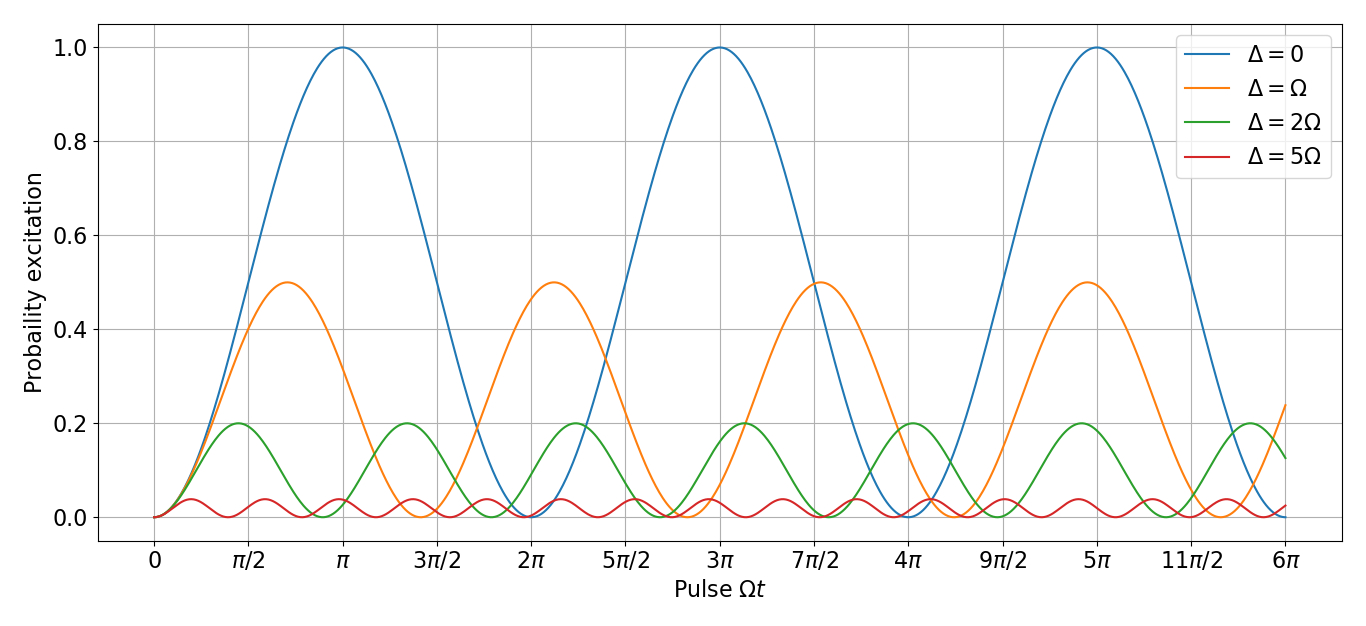
\includegraphics[width = 1\textwidth]{rabiflops}
\caption{Rabi flops for different detuning $\Delta$}
\label{rabiflops}
\end{figure}

Rabi oscillations can be observed with near resonant light, in the off-resonant regime, oscillations are suppressed, but the light shifts the energy levels.
The shift $\delta$ can be calculated by finding the eigenvalues of the Hamiltonian \eqref{Hamiltonianrotatingframe}. It can be easily written in matrix form and diagonalized, we find that there are two eigenstates $\ket{+}$ and $\ket{-}$ called dressed states with eigenvalues
\begin{equation}
E_{\pm} = -\frac{\hbar\Delta}{2} \pm \frac{\hbar}{2}\sqrt{\Delta^2 +\Omega^2}.
\end{equation}
In the limit $\Delta \gg \Omega$, dressed states tend to the bare states $\ket{+} \to \ket{e},\ket{-}\to \ket{g}$, and the energies becomes
\begin{equation}
E_{\pm} \to -\frac{\hbar \Omega}{2} \pm \frac{\hbar \Omega}{2} \pm \frac{\hbar \Omega^2}{4\Delta} \implies \delta = \pm\frac{\Omega^2}{4\Delta}.
\end{equation}
The effective Hamiltonian for the off-resonant regime can be derived following a Markovian approximation \cite{acstarkhamiltonian}
\begin{equation}
H_{eff} = \frac{1}{\hbar \Delta} [\sigma,\sigma^\dagger] = \frac{\hbar \delta}{2}\sigma_z
\end{equation}
The corresponding evolution is
\begin{equation}
\label{acstarkrotation}
U(t) = \exp\left\{-\frac{i}{\hbar} H_{eff} t \right\} =
 \begin{pmatrix}
   \exp\left\{i\frac{\delta}{2}t\right\} & 0\\
   0 & \exp\left\{i\frac{\delta}{2}t\right\}
\end{pmatrix}.
\end{equation}
This matrix implements the quantum gate from equation \eqref{quantumgates}. Furthermore, Ac stark shift can also implement the phase gate \eqref{Hadamard}, the trick is to shift the energy of a transition the shares only one level with qubit transition. From the prospective of the qubit, only one level is shifted and the other level remains unaltered, thus one of the two matrix element of equation \eqref{acstarkrotation} is 1.

\section{Quantum networking with trapped ions}
\subsection{General introduction}
Quantum networks can serve different purposes, either transmission of quantum information at long distances, or interconnections of quantum processors for qubits scaling. The topology of these configurations changes, but the constituent elements are the same: a node, where quantum information is prepared, manipulated, and stored; and a link that connects node and where information is transmitted. Links are typically realized with optical fibers, photons can carry quantum information over long distance with very high speed. Instead, nodes can be realized in a variety of ways: trapped ions \cite{ion_quantumnetwork}, neutral atoms \cite{Ritter2012}, atomic ensembles \cite{kimble}. Nodes and links are connected through an interface that converts deterministically a stationary qubit in a node to a flying qubit over the network. In the next section we will explore how an interface can be realized by placing an ion based quantum memory in a optical cavity. Here we will examine some properties needed for a quantum network to work.\\
In the case of quantum information transmission, a fundamental property of quantum network is the ability of transmitting faithfully any state between nodes. For long distances this requires the use of amplifiers or repeaters that boost the signal as it gets attenuated during the transmission. However, due to the no-cloning theorem \cite{nocloning}, qubits cannot be copied. A workaround of this problem is to send multiple qubits and purify the entanglement along the transmission with extra qubits and quantum nodes between the endpoints \cite{quantumrepeters}.\\
To create a cluster of quantum nodes, another property of quantum network is necessary: entanglement distribution allows to entangle qubits located in different quantum nodes. A protocol to distributed entanglement can be realized with photon interference on a beam splitter. Consider the case of figure \ref{remoteentanglement}. Two nodes each with a qubit
\begin{equation}
\ket{\psi_A} = a\ket{0}_A + b\ket{1}_A \qquad \ket{\psi_B} = c\ket{0}_B + d\ket{1}_B.
\end{equation}
With the use of an interface each qubit is entangled to a photon. The photonic qubit can have different implementations, for this protocol however it is not important and we will indicate them as $\ket{H},\ket{V}$.
The states ready for transmission are
\begin{equation}
\ket{\psi_A} = a\ket{0}_A\ket{H}_A + b\ket{1}_A\ket{V}_A \qquad \ket{\psi_B} = c\ket{0}_B\ket{H}_B + d\ket{1}_B\ket{V}_B.
\end{equation}
The total system is described as the product state of the two subsystem:
\begin{equation}
\ket{\psi_A}\otimes \ket{\psi_B} = (a\ket{0}_A\ket{H}_A + b\ket{1}_A\ket{V}_A)\otimes (c\ket{0}_B\ket{H}_B + d\ket{1}_B\ket{V}_B).
\end{equation}
When the photons arrive at the beam splitter there are four possible outcomes and two distinguishable events: either the two detectors click at the same time or only one detector clicks twice. In the second case, one photon was transmitted and the other reflected, the final state is proportional to $\ket{0}_A \ket{1}_B + \ket{1}_A \ket{0}_B$, which in the case of indistinguishable photons  is just a product state. More interesting is the case when a coincidence on both detector occurs. The final state is projected into
\begin{equation}
\ket{\psi} = ac\ket{0}_A \ket{0}_B + bd\ket{1}_A \ket{1}_B,
\end{equation}
leading to the two qubits to be entangled with each other. This protocol is probabilistic, but the success of entanglement can be heralded after a coincidence measure.
\begin{figure}[H]
  \centering
  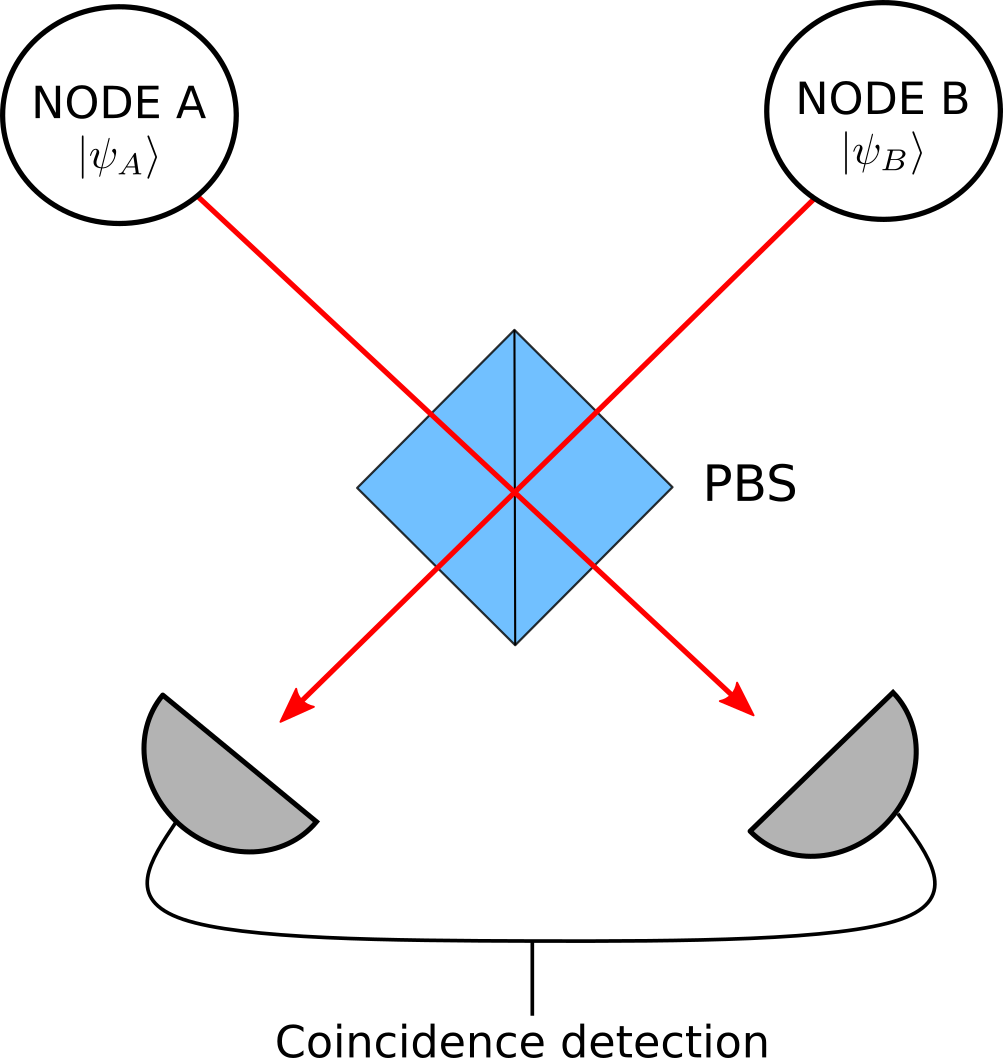
\includegraphics[width = .5\textwidth]{entaglement}
  \caption{Remote qubits entanglement protocol.}
  \label{remoteentanglement}
\end{figure}



\subsection{Cavity QED}
Trapped ions can become quantum nodes of a quantum network by placing them in a cavity. Ions emits photon by spontaneous emission, or stimulated emission. The problem with spontaneous emission is that the photonic channel of emission is random and in free space. To realize a quantum interface, photon should be produces almost deterministically in defined mode. The trick is to use a cavity tuned to one particular transition, such that the probability of a photon to be emitted in the cavity mode is greatly enhanced. In this section we describe a simple model of a two-level system in a cavity, the derivation is similar to section \ref{laserioninteractions}, with the difference that in a cavity the electric field is quantized. Using the mode operator $a,a^\dagger$ the electric field inside a cavity can be written as:
\begin{equation}
E = A(f(r)a + f^*(r)a^\dagger)
\end{equation}
where $A$ is an amplitude, and $f(r)$ is the spatial mode profile \cite{helene}. The interaction between he field and the cavity is obtained as from $H_{int} = -d\cdot E$, following a rotating wave approximation the result is
\begin{equation}
H_{int} = \hbar g (\sigma a^\dagger + \sigma^\dagger a),
\end{equation}
where $g = A \braket{g|d|e} f(r)$ is called cavity coupling constant. It is analogous to the Rabi frequency, it gives an idea of the coupling between the cavity field and the 2-level atom. An important dependence of $g$ can be found by considering that $f(r)$ is inversely proportional to the volume of the cavity $V$, i.e.
\begin{equation}
g \propto \braket{g|d|e} \sqrt{\frac{\omega}{2\varepsilon_0 \hbar V}}.
\end{equation}
The coupling therefore, increases with decreasing cavity volume and viceversa.\\
The total system Hamiltonian includes also the atomic part, and a single mode optical field. It takes the name of Jaynes-Cummings Hamiltonian and it is written as \cite{qedreview}
\begin{equation}
H = \hbar \omega_0 \ket{e}\bra{e} + \hbar \omega a^\dagger a + \hbar g (\sigma a^\dagger + \sigma^\dagger a).
\end{equation}
States now are a product state of the atomic part and the photon number $\ket{g,n},\ket{e,n}$. They are however not the eigenstates of the Jaynes-Cumming Hamiltonian. It can be seen that this Hamiltonian is block diagonal, which means that each $2\times 2$ block can be diagonalized, the dressed states found after diagonalization are similar to the semiclassical model. Moreover, also the dynamics is analogue to the semiclassical case, Rabi oscillations are still present with quantized Rabi frequency given by $\Omega_n = \sqrt{4(n+1)g^2 +\Delta^2}$.\\
The presence of a cavity makes dynamics more interesting, especially when considering spontaneous emission and interaction with cavity modes. For a mathematical description, we need to introduce dissipative process that do not follow an Hermitian evolution. This is done heuristically by adding terms in the Heisenberg equation
\begin{equation}
\label{masterequation}
\frac{d\rho}{dt} = \frac{1}{i\hbar}[H,\rho] + \mathcal{L}(\rho).
\end{equation}
This equation is usually referred to as master equation in Lindblad form, where $\rho$ is the density matrix of system. The superoperator
$\mathcal{L}(\rho)$ contains phenomena not included in the Hamiltonian. In our case, we are most interested in two process: spontaneous emission in a free space field mode, and decay in one cavity mode and out of the cavity. The first is quantified with the decay rate $\Gamma$, while the latter is characterized by the decay rate $\kappa$. The functional dependence of these two terms goes as \cite{steck}
\begin{equation}
\mathcal{L}(\rho) = \Gamma\mathcal{D}(\sigma)\rho + \kappa \mathcal{D}(a)\rho.
\end{equation}
A good approximation of the model is given in the \emph{strong coupling} regime $g\ll \Gamma,\kappa$, where damping due to dissipative process is slow and dynamics is mainly driven coherently by the coupling atom-cavity $g$. The decay rate $\kappa$ depends exclusively on the cavity parameters as \cite{helene}
\begin{equation}
\kappa =\frac{c\pi}{FL},
\end{equation}
where $F$ is the cavity finesse, and $L$ the length. In the design of the experiment one must play and compromise with these three parameters in order to reach a good coupling ion-cavity but also being able to send photons out of the cavity.

\section{Basics of ion trapping}
\subsection{Linear Paul trap}
In order to trap a charged atom, a three dimensional trapping potential $\phi$ is needed. However it follows directly from Maxwell equation $\nabla^2 \phi = 0$ that the potential must be antitrapping at least in one direction. There are two workarounds for this problem: the first one introduces magnetic fields to trap particles in some directions, this takes the name of Penning trap. The second solution is the so called Paul trap, and it is what we are going to describe in this section. The idea is to introduce a time varying potential, such that the antitrapping direction is constantly switching between two  different dimension. If the switching is timed correctly, the particle will not have the time to escape but will always encounter a potential barrier.
The shape of the trap can be adapted to load more ions in different geometries. For instance, a linear Paul trap is elongated in one direction where the trapping confinement is weaker, such that loaded ions will align in a single long string. This kind of trap is depicted in figure \ref{trap}.
\begin{figure}[H]
\centering
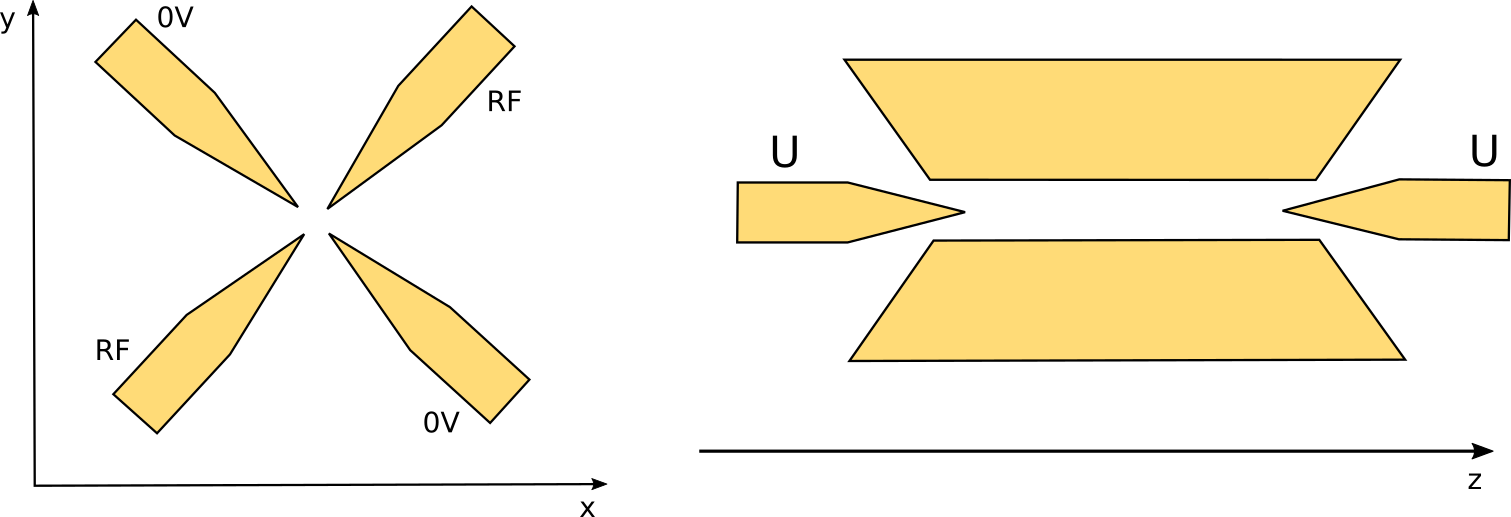
\includegraphics[width = .7\textwidth]{trap}
\caption{A linear paul trap. U is the voltage applied to the electrodes trapping in the $z$ direction, while in the $x-y$ plane trapping is achieved with a radio frequency signal. $r_0$ is the distance from the central axis to the RF electrodes.}
\label{trap}
\end{figure}
The confinement in the $x-y$ plane is provided by 4 electrodes, two of which are grounded and the other two are connected to a radio frequency source. This design is similar to a mass filter, with the difference of additional endcaps electrodes in the $z$ direction that plug the trap and confine also in axial direction.\\
The potential inside the trap can be described for the $x-y$ plan independently from the $z$ direction. In the case of a linear Paul trap the radial potential is \cite{traptheory}:
\begin{equation}
\phi  = \frac{\Phi_0}{2r_0^2}\left(x^2 - y^2\right),
\end{equation}
with the amplitude that consists of a static part $U$ and a dynamical one $\Phi_0 = U + V \cos(\Omega_{RF} t)$.
The study of the particle's motion with mass $m$ and charge $e$ inside the trap can be done with classical physics, Newton's second law in this case is
\begin{equation}
m\ddot{x} = -q \frac{\partial \phi}{\partial x} = - \frac{ex}{r_0^2}\left(U + V \cos(\Omega_{RF} t) \right),
\end{equation}
and similarly for $\ddot{y}$. This equation can be written in the form of Mathieu equation by defining two parameters:
\begin{equation}
a_x = \frac{4eU}{\Omega_{RF}^2r_0^2m}, \quad q_x = \frac{2eV}{\Omega_{RF}^2r_0^2m} \implies \ddot{x} +\frac{\Omega_{RF}}{4} \left(a_x + 2q_x \cos(\Omega_{RF} t )\right)x = 0
\end{equation}
and with a change of variable $\tau = \frac{\Omega_{RF} t}{2}$ we end up with
\begin{equation}
\label{mathieu}
\frac{\partial^2 x}{\partial \tau^2}+\left(a_x + 2q_x \cos(2\tau)\right)x = 0
\end{equation}
This kind of equations have stable solutions that can be found in a recursive way with Floquet theorem \cite{iondynamic}. However, the problem is simplified by performing the so called secular approximation, which consists of separating the motion in a slow changing position: $\bar{x}$ called \emph{secular motion}, and in a rapid oscillation: $\xi$, called \emph{micromotion}. The behaviour of micromotion is dictated by the force due to the potential at the position $\bar{x}$, and the secular motion will follow a time average of the potential $\langle \phi(t) \rangle$ eliminating therefore the effect of micromotion. In this case, equation \eqref{mathieu} can be solved in the limit $a_x \ll q_x \ll 1$
\begin{equation}
x(t) = x_0 \cos(\omega_x t +\phi_x)\left[1 + \frac{q_x}{2}\cos(\Omega_{RF} t) \right].
\end{equation}
Where we recognize a slowly varying oscillation with amplitude modulated by a faster oscillation. The approximation is valid only in the case $\omega_x \ll \Omega_{RF}$. The frequency $\omega_x$ is given in the solution as
\begin{equation}
\omega_x = \frac{\Omega_{RF}}{2}\sqrt{a_x + \frac{q_x^2}{2}}.
\end{equation}
By imposing real solution, the stability diagram of the trap can be found. It is depicted in figure \ref{stabilitydiagram}. The other spatial dimension can be treated in the same way and the results are the same. Important to notice is that a consequence of the secular approximation is that the potential can be approximated, the ion in the trap sees therefore a pseudo potential which is harmonic. Deviations from harmonicity are possible and they are mainly due to stray fields. Extra electrodes can be added to the trap design to compensate for such deviations.


\begin{figure}[H]
\centering
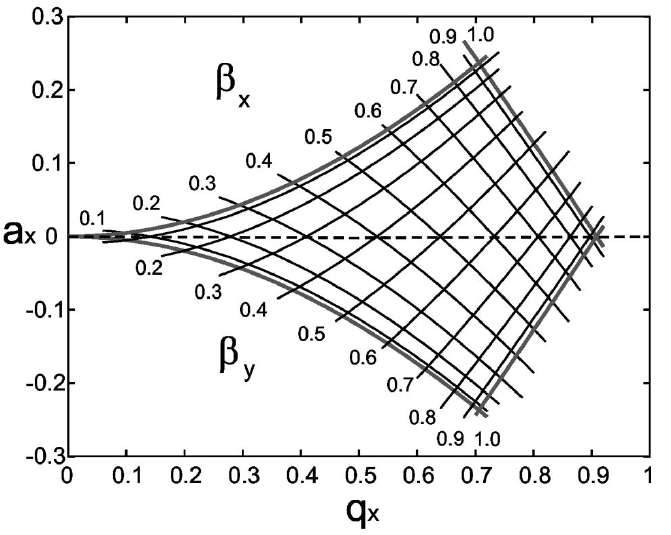
\includegraphics[width = .7\textwidth]{stabilitydiagram}
\caption{Stability diagram for a linear Paul trap, taken from \cite{iondynamic}. The coefficient $\beta_x,\beta_y$ can be calculated numerically from $a_x$ and $q_x$}
\label{stabilitydiagram}
\end{figure}


\subsection{Ion strings}
\label{ionstrings}
We have seen that the potential inside the trap can be described as an harmonic potential. What we are interested in, is the ion separation between $N$ ions loaded in the trap. This will give us an idea of how narrowly the beam should be focused and will set an appropriate problem spatial scale.\\
Let us consider the $z$ direction where the ions are weakly confined and will form a string. The potential can be approximated as harmonic and hence given by
\begin{equation}
V = \sum_{i=0}^N \frac{1}{2}M\omega^2z_i^2 + \sum_{i\neq j}^N\frac{Z^2e^2}{8\pi \epsilon_0}\frac{1}{|z_i-z_j|}
\end{equation}
The equilibrium position can be found at the minima of the potential, i.e. where the first derivative zeros
\begin{equation}
\frac{\partial V}{\partial z_i} = 0 \implies u_i - \sum_{j=1}^{i-1} \frac{1}{(u_i-u_j)^2} + \sum_{j= i+1}^{N} \frac{1}{(u_i-u_j)^2}= 0,
\end{equation}
where we defined the dimensionless quantity $u_i = z_i/l$ and $l^3 = \displaystyle\frac{Z^2 e^2 }{4\pi \epsilon_0 M\omega^2}$.
The last equations can be solved analytically only for 2 or 3 ions. In fact, for the case $N=2$ we simply get the system
\begin{equation}
\begin{cases}
  u_1 + \frac{1}{(u_1-u_2)^2} = 0\\
  u_2 - \frac{1}{(u_1-u_2)^2} = 0
  \end{cases} \quad \implies \quad u_1 = -u_2,\quad  u_1 = \left(\frac{1}{2}\right)^{2/3} \simeq 0.629
\end{equation}
For calcium-40 ions in a Paul trap with axial confinement of $\omega = 1$ MHz, we have $l \simeq 4.45\times 10^{-6}\,$m, which means that 2 ions are separated by $\simeq 5.6\, \mu$m. In the case of more ions the separation is lesser with the same confinement, but it is also possible to lower the axial frequency and increase the separation between the ions such that also in the case of several ions, the distance between them is still in the order of several $\mu$m. This size is accessible with current focusing optics and it is above the diffraction limit.\\
For more ions, a numerical approach has to be used, \cite{ion_spacing} reports values of $u_i$ up to $N=10$, and gives an empirical formula of the minimum separation
\begin{equation}
u_{min}(N) \simeq \frac{2.018}{N^{0.559}},
\end{equation}
Although, numerical solution are preferred and can be computed fast.
\subsection{Doppler cooling and detection}
Ion trapping was treated here classically, because ions, when trapped, are still hot and follow classical mechanics. In order to reach the quantum regime, they must be cooled down. Several techniques are available for cooling, but the most popular and more frequently used is doppler cooling. The idea comes from neutral atoms and can be applied to ions as well: a laser interacts with a particular transition, exchanging a photon and therefore giving a momentum kick $\Delta p = \hbar \mathbf{k}$ in a particular direction to the ion. The absorbed photon is given back through spontaneous emission in a random direction, giving another kick to the ion. Over many cycles of absorption and emission, the random kick due to emission will average to zero, while the kick given by the laser will accumulate slowing down and cooling the ion in the direction of the laser. \\
The difference with neutral atoms is that an ion is confined inside a trap rotating at frequency $\omega$. Hence, even the simple 2-level system gains new transitions called sidebands. Some consideration must be put into the relative strength of the decay rate $\Gamma$ with respect to the sidebands. For describing the Doppler cooling we assume that the ion is weakly confined $\omega \ll \Omega$. The intuitive picture is that the rate of spontaneous emission in this case is much faster that the time scale over which the trap changes potential. Therefore, the trap can be considered static  and has no effect on the cooling.\\
In order to describe spontaneous emission, we use the master equation \eqref{masterequation}, in the case of spontaneous emission, the superoperator is given by \cite{gabriel}
\begin{equation}
\mathcal{L}(\rho) = \frac{\Gamma}{2}\left(2\sigma \rho \sigma^\dagger - \left\{\sigma^\dagger \sigma, \rho\right\}\right).
\end{equation}
$\Gamma$ is the decay rate from the excited state to the ground state. The actual value is found in perturbation theory with Fermi's golden rule []
\begin{equation}
\Gamma = \frac{\omega_0^3}{3\pi \varepsilon_0 \hbar c^3} |\braket{e|d|g}|^2
\end{equation}
The master equation \eqref{masterequation} can be explicitly written for every component of the density matrix $\rho$, in the rotating frame they are called optical equations and they are
\begin{equation}
\label{rhoee}
\frac{d\rho_{ee}}{dt} = -i\frac{\Omega}{2}(\rho_{eg} - \rho_{ge}) - \Gamma \rho_{ee}
\end{equation}
\begin{equation}
\frac{d\rho_{gg}}{dt} = i\frac{\Omega}{2}(\rho_{eg} - \rho_{ge}) + \Gamma \rho_{ee}
\end{equation}
\begin{equation}
\frac{d\rho_{ge}}{dt} = -\left(\frac{\Gamma}{2}+i\Delta\right)\rho_{ge} -i\frac{\Omega}{2}(\rho_{ee} - \rho_{gg})
\end{equation}
\begin{equation}
\frac{d\rho_{eg}}{dt} = -\left(\frac{\Gamma}{2}-i\Delta\right)\rho_{eg}+i\frac{\Omega}{2}(\rho_{ee} - \rho_{gg})
\end{equation}
The most interesting solution is the population of the excited level $\rho_{ee}$ in the steady state case, i.e. when the system reached he equilibrium. In this case we look at $\rho_{ee}(t\to \infty) $, the solution of equation \eqref{rhoee} is
\begin{equation}
\rho_{ee}(t\to \infty) = \frac{\Omega^2/\Gamma^2}{1 + \left(2\frac{\Delta -\mathbf{k}\cdot \mathbf{v}}{\Gamma}\right)^2 + 2\frac{\Omega^2}{\Gamma^2}}
\end{equation}
The force exerted on the ions, due to the radiative pressure, is proportional to this population as
\begin{equation}
F = \hbar k \Gamma \rho_{ee} \simeq F_0 + \frac{dF}{dv}v = \hbar k \Gamma\frac{\Omega^2}{\Gamma^2 +4\Delta^2} + F_0 \frac{8k\Delta}{\Gamma^2 + 4\Delta^2}v
\end{equation}
where we assumed low velocities $v \simeq 0$ and thus linearized the equation. The effect of the constant term in the force is just to displace the ion from its central position. Instead, the linear term acts as a viscous friction that cools the ions with a rate of $\dot{E}_c = \braket{Fv}$.
If on one side spontaneous emission allows for Doppler cooling, it also sets the lower limit. The small fluctuations in the Brownian motion leads to diffusion which heats the ion at a rate of
\begin{equation}
\dot{E}_h = \frac{1}{m}\frac{d}{dt}\braket{p^2} =  \frac{1}{m}(\hbar k)^2 \Gamma \braket{\rho_{ee}(v)}.
\end{equation}
At equilibrium, the heating rate equals the cooling rate giving the lowest temperature achievable
\begin{equation}
\dot{E}_h + \dot{E}_c = 0  \implies k_B T = -\frac{\hbar \Gamma}{4}\left(\frac{\Gamma}{2\Delta} +\frac{2\Delta}{\Gamma}\right).
\end{equation}
From here it is clear that by choosing the appropriated detuning, it is possible to reach the lowest temperature
\begin{equation}
T_{min} = \frac{\hbar \Gamma}{2k_{B}}, \qquad \text{for} \quad \Delta = -\frac{\Gamma}{2}
\end{equation}
The achieved temperatures with Doppler cooling are enough to perform standard measurements. To go further down in temperature, sideband cooling is used, here particular sideband transition are excited to reduce the phonon number of the ions inside the trap.\\
With the same interaction of Doppler cooling, state detection can also be performed by means of laser induced fluorescence. Consider the $\Lambda$ scheme in figure \ref{threelevel}, the qubit is encoded in the level $\ket{g_1}$ and $\ket{g_2}$. To distinguish in which state the electron is, the transition $\ket{g_1}\to \ket{e}$ is excited. In the case the electron is in $\ket{g_1}$, the electron undergoes Rabi flops and scatters photons that can be collected and measured. If the electron is $\ket{g_2}$, no photons will be emitted and therefore no light is collected. The difference between these bright and dark states is clear and detection can be performed efficiently with near perfect efficiency.\\
In the real case, one must take into consideration also all the other levels. In fact, an electron from the excited state $\ket{e}$ can have multiple decay channels to other states and repumping becomes necessary.
\begin{figure}
\centering
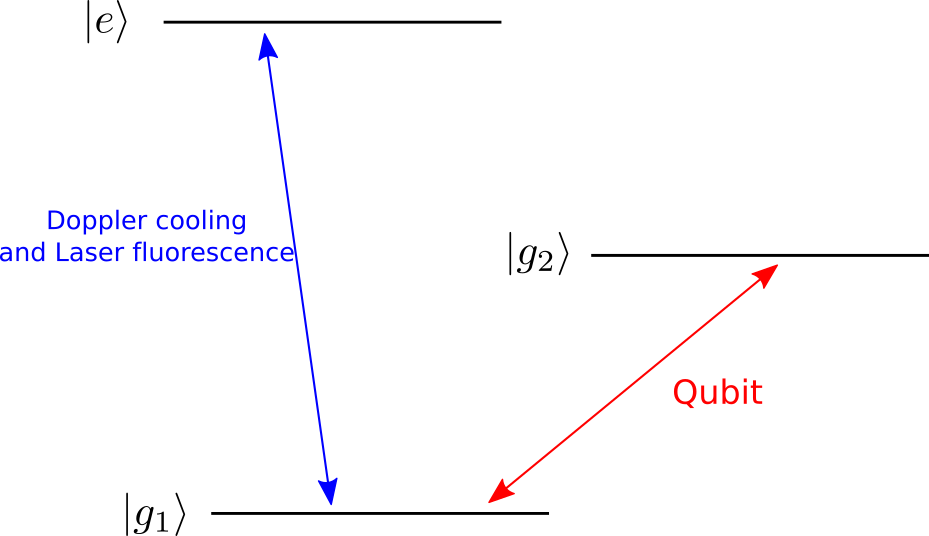
\includegraphics[width = .6\textwidth]{threelevelatom}
\caption{$\Lambda$ type scheme. Two ground states $\ket{g_1}$ and $\ket{g_2}$ are stable or metastable, while the excited level $\ket{e}$ is short lived. Qubit is encoded in the two ground states while laser fluorescence and laser cooling is done on the $\ket{g_1}\to \ket{e}$ transition.}
\label{threelevel}
\end{figure}
\section{Laser beam}
\subsection{Gaussian beams}
\label{sec_diffraction}
Lasers emit light in the shape of Gaussian beams, so it is import to understand what Gaussian beams are and their characteristics. In this chapter we will take a closer look into such beams and introduce important quantities to characterize a Gaussian beam. \\
From a theoretical point of view, Gaussian beams are solution of the Helmholtz equation $(\nabla^2 + k^2)U(r) = 0$, with $k$ being the wavevector. Such equation is a time independent variant of the wave equation that follows directly from Maxwell equations. A paraxial approximation is often used, i.e.  we assume that the amplitude $A(r)$ of the wave is slowly varying, this means that the envelope of the wave is approximately constant on a length of $\lambda$ and we can write the complex electric field as $U(r) = A(r)e^{-ikz}$. If we can consider a wave propagating in the $z$ direction, we can find a solution in the form of \cite{saleh}:
\begin{equation}
\label{gaussianbeams}
U(r) = A_0 \frac{W_0}{W(z)}\exp\left\{-\frac{x^2+y^2}{W^2(z)}\right\}\exp\left\{-ikz-ik\frac{x^2+y^2}{2R(z)}+i\arctan(z/z_0)\right\}.
\end{equation}
 These solutions are called Gaussian beams, they are characterized by an amplitude $A$, a width $W(z)$, Rayleigh range $z_0$, and a curvature radius $R(z)$. Let us take a look at the features that arise from these beams. The optical power can be calculate by taking the square of the complex amplitude
\begin{equation}
\label{beamintensity}
I(r) = |U(r)|^2 = I_0 \left(\frac{W_0}{W(z)}\right)^2 \exp\left\{\frac{2x^2 + 2y^2}{W^2(z)}\right\}  \qquad I_0 = |A_0|^2.
\end{equation}
It is clear from here why the beam is called Gaussian. For a fixed $z$, the beam shape is the one of a two dimensional beam profile, i.e. the sections in the $x-y$ plane of a Gaussian beams are Gaussian shaped distribution. If we further take a cross section in the $x-y$ plane, we end up with a one dimensional Gaussian distribution. This shape is shown in figure \ref{gauss}, along with some important parameters.
\begin{figure}
\centering
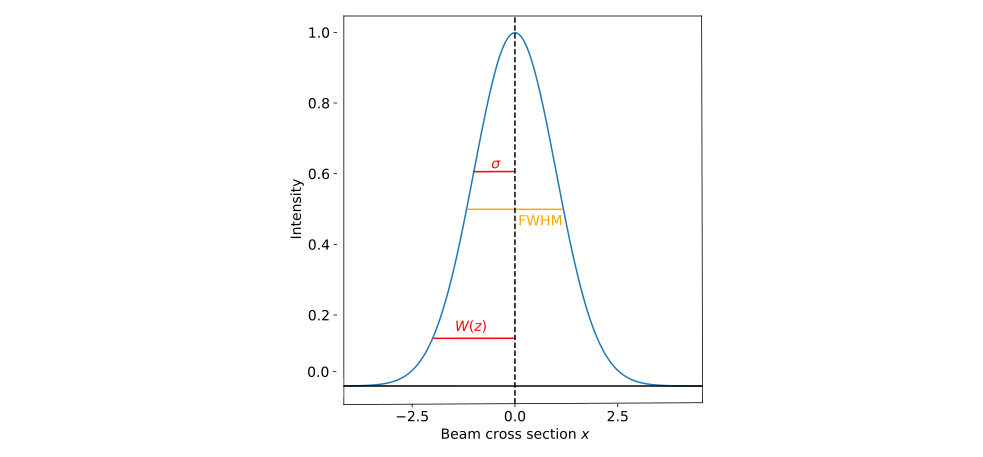
\includegraphics[width = .6\textwidth]{gauss}
\caption{Normalized Gaussian profile. Different ways of measuring the width of the profile are displayed geometrically.}
\label{gauss}
\end{figure}
It is important to understand how to characterize the width of a Gaussian shape, as it provides a quantitative way of measuring a laser beam width and its focus spot. A common way to define the width of a Gaussian distribution is according to the standard deviation $\sigma$, in this case the shape is given by $Ae^{-\frac{x^2}{2\sigma^2}}$, but for the intensity of a Gaussian beam, $W(z)$ is a much more used value. $W(z)$ is defined as the point at which the irradiance $I$ has fallen to $1/e^2 = 13.5\%$ of its maximum value. The relationship between these two quantities is easily found: $W(z) = 2\sigma$.\\
Another common parameter to characterize the width of a Gaussian is the full width half maximum (FWHM), this can be found to be related to $W$ as: $W = 0.84\cdot \text{FWHM}$. All these methods are equivalent and are different only from a prefactor, so for the rest of the section, we can stick to $W(z)$ and study its behaviour. Always from Helmholtz equation \cite{saleh}, the profile of $W(z)$ is found to be
\begin{equation}
\label{waistprofile}
W(z) = W_0 \sqrt{1 + \left(\frac{z}{z_0}\right)^2}\qquad W_0 = \sqrt{\frac{\lambda z_0}{\pi}}.
\end{equation}
This equation is plotted in figure \eqref{gaussprofile}.
\begin{figure}
\centering
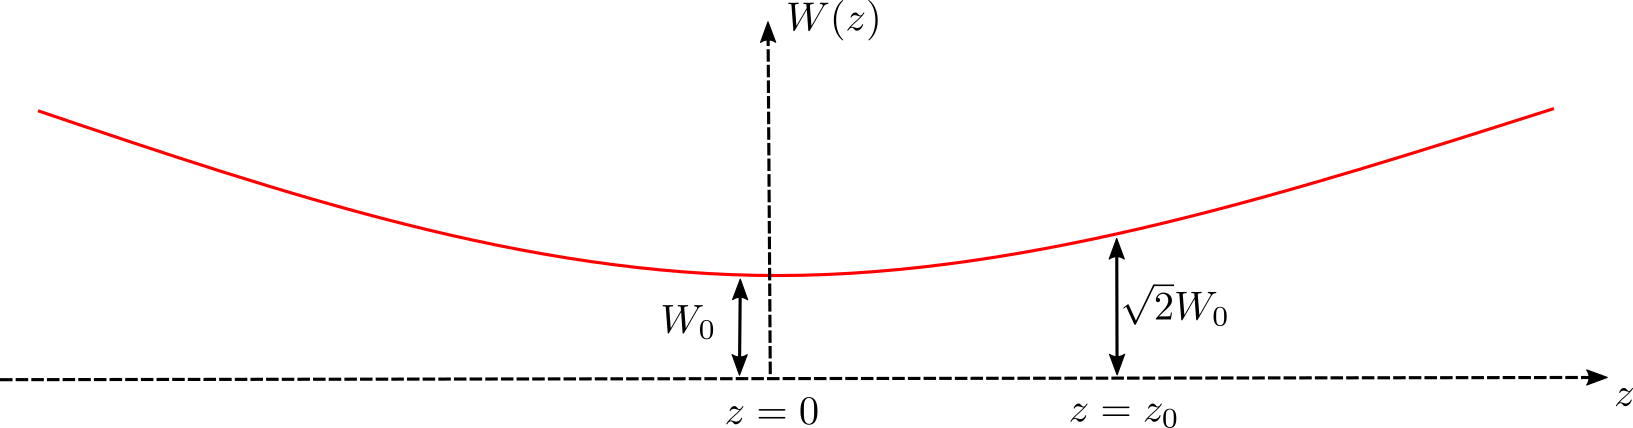
\includegraphics[width = \textwidth]{gaussprofile}
\caption{Width profile of a Gaussian beam. The beam is focused at the position $z_0$, here it assumes the minimum width $W_0$, also referred to as waist.}
\label{gaussprofile}
\end{figure}
There are several important features that can be seen. First of all, the width reaches a minimum in $z=0$ at a value of $W_0$, this is called focus of the beam and its width is the waist of the beam. Before and after the focus, the beam profile diverges almost linearly with an angle given by $\theta = W_0/z_0$, which means the smaller the focus, the greater it diverges. This property will become important later in the work, because it provides one limit on the focus spot. In fact, the optical aperture of the trap is limited by the electrodes, and a too diverging beam can potentially clip on one electrode causing aberrations and scattered light in the whole trap.  The Rayleigh range $z_0$ also has a geometrical interpretation, it represents the point where the beam width is exactly $\sqrt{2}W_0$, along with $\theta$ this is a useful way to characterize how fast a beam diverges.\\

In real experiments, all of these beam quantities can be manipulated with a lens. A Gaussian beam can therefore be shaped at will using optical elements. In order to study such reshaping, let us consider a thin spherical lens with focal length $f$, and radius of curvature $R_l$ placed at position $z$. The effect of the lens on the beam is to give an extra phase factor to equation \eqref{gaussianbeams} equals to $k(x^2 + y^2)/2f$ \cite{beamparameters}. We can match the phase of the incoming and emerging waves
\begin{equation}
kz +k \frac{x^2+y^2}{2R} - \zeta  - k\frac{x^2 + y^2}{2f} = kz + k \frac{x^2+y^2}{2R'} - \zeta \implies \frac{1}{R'} = \frac{1}{R} - \frac{1}{f}.
\end{equation}
The effect of the lens is now clear, it changes the radius of curvature to $R'$ according to the previous equation. Moreover, the width of the beam at the lens is not altered $W=W'$. Using these last two facts, we can determine all the parameters of the outgoing wave. The most important for us is the new waist $W_0'$
\begin{equation}
W_0' = MW_0 \qquad M = \frac{M_r}{\sqrt{q+r^2}} \qquad M_r = \left|\frac{f}{z-f}\right| \qquad r = \frac{z_0}{z-f}.
\end{equation}
$M$ is the magnification factor which provides an easy way to describe the change of the beam. For a better understanding of this last result, let us consider an less general example. We can place the lens at the focus $z=0$, and have a collimated beam $z_0 \to +\infty $. In this case the new waist is
\begin{equation}
W_0' = \frac{W_0}{\sqrt{1 + (z_0/f)^2}} \simeq W_0\frac{f}{z_0} = \frac{\lambda f}{\pi W_0}
\end{equation}
where the approximation comes from taking $z_0\gg f$. There are three parameters we can act on to achieve the smallest focus spot. The wavelength $\lambda$, the shorter the better. The focal length of the lens $f$ must be as small as possible, and the waist of the incoming beam $W_0$ as big as possible. Usually the wavelength is fixed in an optical system, so the best way to achieve a small focus is to collimate the beam as large as possible, the limit is given by the diameter $D$ of the lens. Hence, in the best case we have $D = 2W_0$ which means the waist is
\begin{equation}
W_0 = \frac{2\lambda}{\pi} \frac{f}{D}.
\end{equation}
A system focused to this limit is said to be diffraction limited. Indeed, if the size of the collimated beam is yet increased, the lens becomes a finite size aperture and diffraction effects will appear at the image plane.% The next section will delve a little bit deeper in this kind of effects since it is the main limitation for the best achievable spot size.

%\subsection{Diffraction limit}
%There are some fundamental limits on how narrow a Gaussian beam can be focused, in this section we will take a look at what is the best achievable focus spot in the theoretical case with the best optics possible.
%- To search whats limiting the diffraction, (lambda/2)
\subsection{Beam stearing via AOD's}
\label{theory_AOD}
Acousto-optical deflectors are a common practical devices to steer a laser beam. Their working principle is based on the Acousto-optical effect. A crystal is strained due to a acoustic wave. A piezo is used to create vibrations that propagate in the crystal, and it is absorbed on the opposite facet of the crystal. Vibrations compress and stretch the medium creating a pattern. Due to the different density of the crystal medium at different position, the refractive index is modified creating a grating that can be used to deflects light.\\
As a simple model, let us consider a rectangular crystal like in figure \ref{AOD}. The acoustic wave creates a sinusoidal pattern with frequency $\Omega_s$ and wavevector $q$, for the refractive index $n(x,t)$
\begin{equation}
n(x,t) = n - \Delta n_0 \cos \left(\Omega_s t - qx \right),
\end{equation}
where $n$ is the refractive index of the unperturbed medium, $\Delta n_0$ is the amplitude of the perturbation. $\Delta n_0$ is proportional to the square root of the sound intensity.

\begin{figure}[H]
\centering
\includegraphics[width = .5\textwidth]{aod}
\caption{AOD.}
\label{AOD}
\end{figure}
The reflected wave can be calculated by dividing the crystal in thin layers, each with his refractive index $n(x)$. The total reflection is given by all the contributions $\frac{dr}{dx}$ of every layer, we can therefore integrate over a length $L$ as follow:
\begin{equation}
r = \int_{L/2}^{L/2} e^{i2kx \sin\theta} \frac{dr}{dx} \,dx
\end{equation}
The included phase takes into consideration the different phase of the input beam when different layers are met. The integral can be solved with a change of variable
\begin{equation}
\frac{dr}{dx} = \frac{dr}{dn}\frac{dn}{dx} = \frac{dr}{dn} q \Delta n_0 \sin \left(\Omega_s t - qx \right),
\end{equation}
The sine function can be written as exponential and now the integral contains only exponential functions which are trivial to calculate. At the end we obtain two contributes for the reflected wave $r$:
\begin{equation}
\label{mainAOD}
r = r_+ + r_- \qquad r_\pm = \pm i r_0 \text{sinc} \left[(2k\sin\theta \mp q)\frac{L}{2\pi} \right]e^{\pm i\Omega_s t}
\end{equation}
These two terms are the plus and minus first order diffraction, an acousto-optical device can be operated symmetrically entering either with a positive angle or with a negative one. Since the maths and the physics is the same, we will focus only on the positive term, called upshifted Bragg diffraction. The sinc function peaks sharply when its argument is 0, i.e. at $2k\sin\theta = q$, and then quickly decreases as the angle is changed. Hence, the input beam must enter with a particular angle in order to diffract. The condition to be satisfied is usually called Bragg condition, and can be written as a function of the wavelengths as
\begin{equation}
\label{braggcondition}
\sin \theta  = \frac{\lambda}{2 \Lambda_s} \qquad \Lambda_s = \frac{2\pi}{q}.
\end{equation}
If the condition is not perfectly matched, some light will not be diffracted and will be transmitted unaltered through the device.
The ration of the transmitted and diffracted light is called diffraction efficiency and gives an idea of how well an acousto-optical device is performing.\\
From equation \eqref{mainAOD} we can notice that an extra phase factor proportional to $\Omega_s t$ is added to the reflected wave. Thus, if the incoming wave is oscilalting at $\propto e^{i\omega t}$, the diffracted wave will oscillate as $\propto r_{+}e^{i\omega t} \implies \propto e^{i(\omega + \Omega_s )t}$. The frequency of the diffracted wave $\omega_r$ is therefore shifted by the frequency of the acoustic vibration as
\begin{equation}
\omega_r  =  \omega + \Omega_s.
\end{equation}
This fact already suggests an application for acousto devices: they can be used as tuning device to shift the frequency of a laser. This kind of devices are called acousto-optical modulator (AOM). However, it is not the only application, we can also use the same device to deflect a beam. The idea is to change the deflection angle $\theta$ by changing the frequency $\Omega_s$ applied to the crystal.
Assume that the angle $\theta$ is small enough to approximate $\sin\theta \sim \theta$, the Bragg condition can be written as
\begin{equation}
\theta \simeq \frac{\lambda}{2 v_s}f,
\end{equation}
where $v_s$ is the speed of sound and $f$ the frequency of the signal. We can already see that if we change the frequency $f$, the deflection angle $\theta$ changes proportionally. Although the Bragg condition \eqref{braggcondition} is not satisfied anymore, we can work with small enough angles that the diffraction efficiency remain above a certain thresholds. The bandwidth is defined as the possible scanning angles, if $B$ is the frequency bandwidth in which the diffraction efficiency stay above a certain number (50\% for instance). Then, the range of scannability is
\begin{equation}
\Delta\theta = \frac{\lambda B}{2v_s}
\end{equation}
there are several way to engineer such device to increase bandwidth and keep the Bragg condition verified, for example the transducer is replaced by a phase array of transducers that tilt the acoustic beam [].
